\chapter{Tecnoloxías e ferramentas}
\label{chap:ferramentas}

\lettrine{N}{este} capítulo falarase das diferentes tecnoloxías e ferramentas empregadas para o desenvolvemento do traballo:
a linguaxe de programación e o seu ecosistema, a librería gráfica empregada nos frontends
e as ferramentas que sosteñen o fluxo de traballo do proxecto.
Pecharase o capítulo cunha xustificación da elección destas tecnoloxías
en relación cos obxectivos do proxecto.

\section{Rust como linguaxe de programación}
Rust é unha linguaxe de programación iniciada como proxecto persoal de Graydon Hoare en 2006,
desenvolvida despois baixo o patrocinio de Mozilla e cunha primeira versión estable publicada en 2015 % \cite{Rust}.

O seu obxectivo era crear unha linguaxe rápida e eficiente,
capaz de render en contornos de programación de sistemas onde se usa principalmente C ou C++,
pero evitando os erros típicos de seguridade na xestión da memoria comúns nesas linguaxes.
Para acadar isto sen necesidade de empregar recolectores de lixo,
demasiado custosos en programas onde o rendemento é un requisito crítico,
emprégase o modelo de pertenza ou \textit{ownership}.

\subsection{Modelo de pertenza e \textit{borrow checker}}
Baixo este modelo, cada valor do programa ten unha única variable dona.
Cando a dona sae do seu ámbito, o valor libérase automaticamente,
seguindo o patrón \acrfull{raii}:
a memoria e o resto de recursos vincúlanse ao tempo de vida das variables,
polo que a súa liberación é determinista e non require intervención do programador.
Asignar un valor a outra variable ou pasalo como argumento implica mover a pertenza,
quedando a variable orixinal invalidada.
Para acceder a un valor sen tomar a súa pertenza empréganse os préstamos ou \textit{borrowing}
, que permiten crear referencias a un valor, mantendo a súa dona orixinal.
Poden existir simultaneamente varias referencias de só lectura, ou ben unha única referencia mutable,
pero nunca ámbalas dúas.
Estas regras de exclusividade non só prevén os accesos inválidos á memoria
, xa que combinadas cos \textit{traits} \texttt{Send} e \texttt{Sync}
, que indican que tipos poden transferirse ou compartirse entre fíos
, eliminan tamén as condicións de carreira en tempo de compilación.
Isto foi denominado pola comunidade como \textit{fearless concurrency}.

O encargado de facer cumprir estas regras é un subsistema do compilador de Rust,
o \textit{borrow checker}.
Este asocia a cada referencia un tempo de vida (\textit{lifetime})
e comproba que ningunha referencia sobreviva ao valor ao que apunta
nin incumpra as regras de exclusividade dos préstamos.
Conceptualmente realiza un labor semellante ao dos analizadores estáticos empregados con C ou C++
, pero incrustando as regras na semántica da linguaxe
, facendo unha análise exhaustiva de forma obrigatoria en tempo de compilación
, en lugar de ser unha ferramenta externa, opcional e baseada en heurísticas.

\subsubsection{Punteiros intelixentes}
Cando as regras de pertenza resultan demasiado restritivas para expresar certos patróns,
como a pertenza compartida ou os grafos con ciclos,
a biblioteca estándar ofrece punteiros intelixentes que as flexibilizan
sen abandonar as garantías da linguaxe:
\texttt{Box} para a asignación en \textit{heap} con pertenza única,
\texttt{Rc} e \texttt{Arc} para a pertenza compartida mediante contadores de referencias,
e \texttt{RefCell} ou \texttt{Mutex} para a mutabilidade interior,
que traslada a comprobación das regras de préstamo do tempo de compilación ao de execución.

Este modelo garda unha relación directa coas boas prácticas do C++ moderno.
No C++ clásico a memoria xestiónase manualmente cos métodos \texttt{new} e \texttt{delete},
fonte de fugas de memoria e de accesos inválidos.
Para mitigalo, o C++ moderno adoptou o patrón \acrshort{raii}
e punteiros intelixentes análogos aos de Rust, como son 
\texttt{unique\_ptr}, \texttt{shared\_ptr} e \texttt{weak\_ptr}.
A diferenza fundamental é que en C++ estas prácticas son convencións opcionais
que o compilador non pode facer cumprir,
mentres que en Rust forman parte da semántica da linguaxe
e a súa violación é un erro de compilación.

\subsubsection{Palabra clave \texttt{unsafe}}
Nos contextos que non poden seguir as regras de Rust debido á súa natureza
, como o acceso directo a hardware, a interoperabilidade con código C
ou certas estruturas de datos altamente optimizadas
, Rust ofrece os bloques \texttt{unsafe}.
Neles o programador asume a responsabilidade de manter as garantías da linguaxe.
Este mecanismo permite manter a localidade das zonas perigosas
facendo posible crear interfaces seguras ao seu redor illando o resto do programa.


\subsection{Sistema de tipos e expresividade}
Ademais do seu innovador modelo de xestión de memoria, Rust busca ser unha linguaxe cómoda e moderna,
incorporando características propias de linguaxes funcionais, como OCaml.
Esta influencia non é casual xa que o primeiro compilador de Rust escribiuse precisamente en OCaml,
antes da reescritura do compilador en Rust.
Podemos atopar esta influencia na existencia de \textit{units} e \textit{tuples}
e na súa orientación a expresións.
Case todas as construcións devolven un valor,
incluídos os bloques, os condicionais e o \textit{pattern matching},
aínda que mantén unha sintaxe de estilo imperativo, familiar para quen procede de C ou C++,
en lugar da sintaxe da familia ML.

Os tipos suma (\texttt{enum}) permiten definir variantes que transportan datos,
sobre as que o compilador esixe un tratamento exhaustivo no \textit{pattern matching}.

Os xenéricos en Rust permiten definir tipos e funcións parametrizados por outros tipos
aforrando código repetitivo e aumentando a súa reutilización sen custos de execución.
A diferenza dos \textit{templates} de C++, que se verifican unicamente ao instancialos
, os xenéricos de Rust permiten restrinxir os tipos que poden empregarse mediante os \textit{traits}.
O compilador verifica se o tipo empregado cumpre con estas restricións en tempo de compilación.

Empregando estes mecanismos Rust crea dous dos tipos máis importantes do seu ecosistema: \texttt{Option} e \texttt{Result}.

\begin{description}
  \item[\texttt{Option}] representa un valor que pode estar presente ou ausente
  , evitando o uso de punteiros nulos e os erros que deles se derivan.

  \item[\texttt{Result}] representa o resultado dunha operación que pode fallar,
  transportando o valor de éxito ou o erro producido. Este tipo é a base do sistema de xestión de erros
  que substitúe as excepcións polos erros como valores,
  deixando as excepcións (en Rust denominadas \textit{panics}) para situacións excepcionais e irrecuperables.
  Ademáis este tipo engade azucre sintáctico para a propagación de erros mediante o operador \texttt{?},
  permitindo escribir código de tratamento de erros conciso e lexible.
\end{description}


\subsubsection{Orientación a obxectos}
Rust afástase tamén da orientación a obxectos clásica ao non existir clases nin herdanza.
Os datos defínense en \texttt{structs} e o comportamento engádese por separado
en bloques \texttt{impl}, que conteñen os seus métodos.
As interfaces compartidas exprésanse mediante \textit{traits},
que un tipo pode implementar para adquirir un comportamento común,
con soporte tanto para o despacho estático, resolto por monomorfización,
como para o dinámico a través dos \textit{trait objects} (\texttt{dyn}).
Foméntase así a composición sobre a herdanza.
Reutílizase código combinando tipos que conteñen outros tipos
e implementando \textit{traits}, que poden ofrecer métodos por defecto,
evitando as fráxiles xerarquías profundas de clases.

\subsubsection{Metaprogramación}
Para completar a súa capacidade expresiva, Rust conta cun sistema de metaprogramación baseado en macros.
Este sistema axuda a reducir o código repetitivo e a xerar implementacións de forma automática,
permitindo expandir a funcionalidade dos nosos tipos sen custo para o programador.
A diferenza do preprocesador de C, que realiza unha substitución textual cega
previa á compilación e allea á linguaxe,
as macros de Rust operan sobre a estrutura sintáctica do código
, polo que non poden capturar accidentalmente variables do contexto onde se expanden,
e o código que producen valídase co resto do programa,
detectándose nel os erros de sintaxe e de tipos e mantendo todas as garantías do compilador.
O seu principal inconveniente é que constitúen unha sublinguaxe propia máis difícil de ler e depurar.


\section{Cargo e o seu ecosistema}
Boa parte da experiencia de uso de Rust débese a Cargo,
o xestor de paquetes e sistema de construción oficial da linguaxe.
Cargo encárgase de descargar e compilar as dependencias do proxecto,
os \textit{crates}, publicados no rexistro central crates.io. % \cite{cratesio}
As dependencias decláranse no manifesto \texttt{Cargo.toml} mediante versionado semántico,
e as versións exactas resoltas quedan fixadas no ficheiro \texttt{Cargo.lock},
o que garante que todas as máquinas compilen exactamente o mesmo código.

Cargo permite ademais organizar varios crates relacionados nun \textit{workspace} común,
que comparte a resolución de dependencias e o directorio de compilación.
Este proxecto está estruturado deste xeito
, cun crate central co núcleo do emulador e crates separados para cada frontend,
como se detallará no capítulo~\ref{chap:implementacion}.

O ecosistema complétase cunha serie de ferramentas oficiais e de terceiros.
Cargo inclúe subcomandos para xestionar dependencias, crear proxectos e compilar e executar tanto o proxectos como as súas probas.
Para outras tarefas, pódense incluir subcomandos externos, que permiten ampliar a funcionalidade de Cargo.

\textit{rustfmt}, \textit{clippy} son o formatador e o linter oficiais, para manter un código limpo e con estilo consistente.
Neste proxecto tamén usamos \textit{cargo-flamegraph} que permite dende a interface de Cargo xerar gráficos
a partir dos datos obtidos empregando o perfilador \textit{perf} de Linux.

\section{Raylib como librería gráfica}
Raylib % \cite{raylib}
é unha librería escrita en C99 e creada por Ramon Santamaria (Raysan5) para crear videoxogos de forma sinxela.
Naceu nun contorno docente, como ferramenta para ensinar programación de videoxogos
a estudantes con pouca experiencia previa en programación,
Ese espírito mantense no seu deseño ofrecendo unha interface sinxela e autocontida para xestionar a ventá, a entrada,
o debuxado e o audio, sen necesidade de empregar a un motor de xogos grande e complexo.

A figura~\ref{fig:raylib-architecture} amosa a súa arquitectura interna,
organizada en módulos independentes.
O módulo central, rcore, xestiona as peculiaridades da plataforma empregada como a creación da ventá,
o contexto gráfico, a entrada e o bucle principal.
Sobre el sitúanse os módulos de debuxado de formas, texturas, texto e modelos 3D,
que non chaman directamente á API gráfica do sistema,
senón a unha capa intermedia, rlgl,
que abstrae as diferentes versións de OpenGL dispoñibles en cada plataforma.
O audio xestiónao o módulo raudio, construído sobre miniaudio.
Precisamente unha das vantaxes da librería é o seu reducido número de dependencias:
as que precisa, como a propia miniaudio, van incluídas no seu código fonte,
variando unicamente en función da plataforma de destino.

\begin{figure}[hp!]
  \centering
  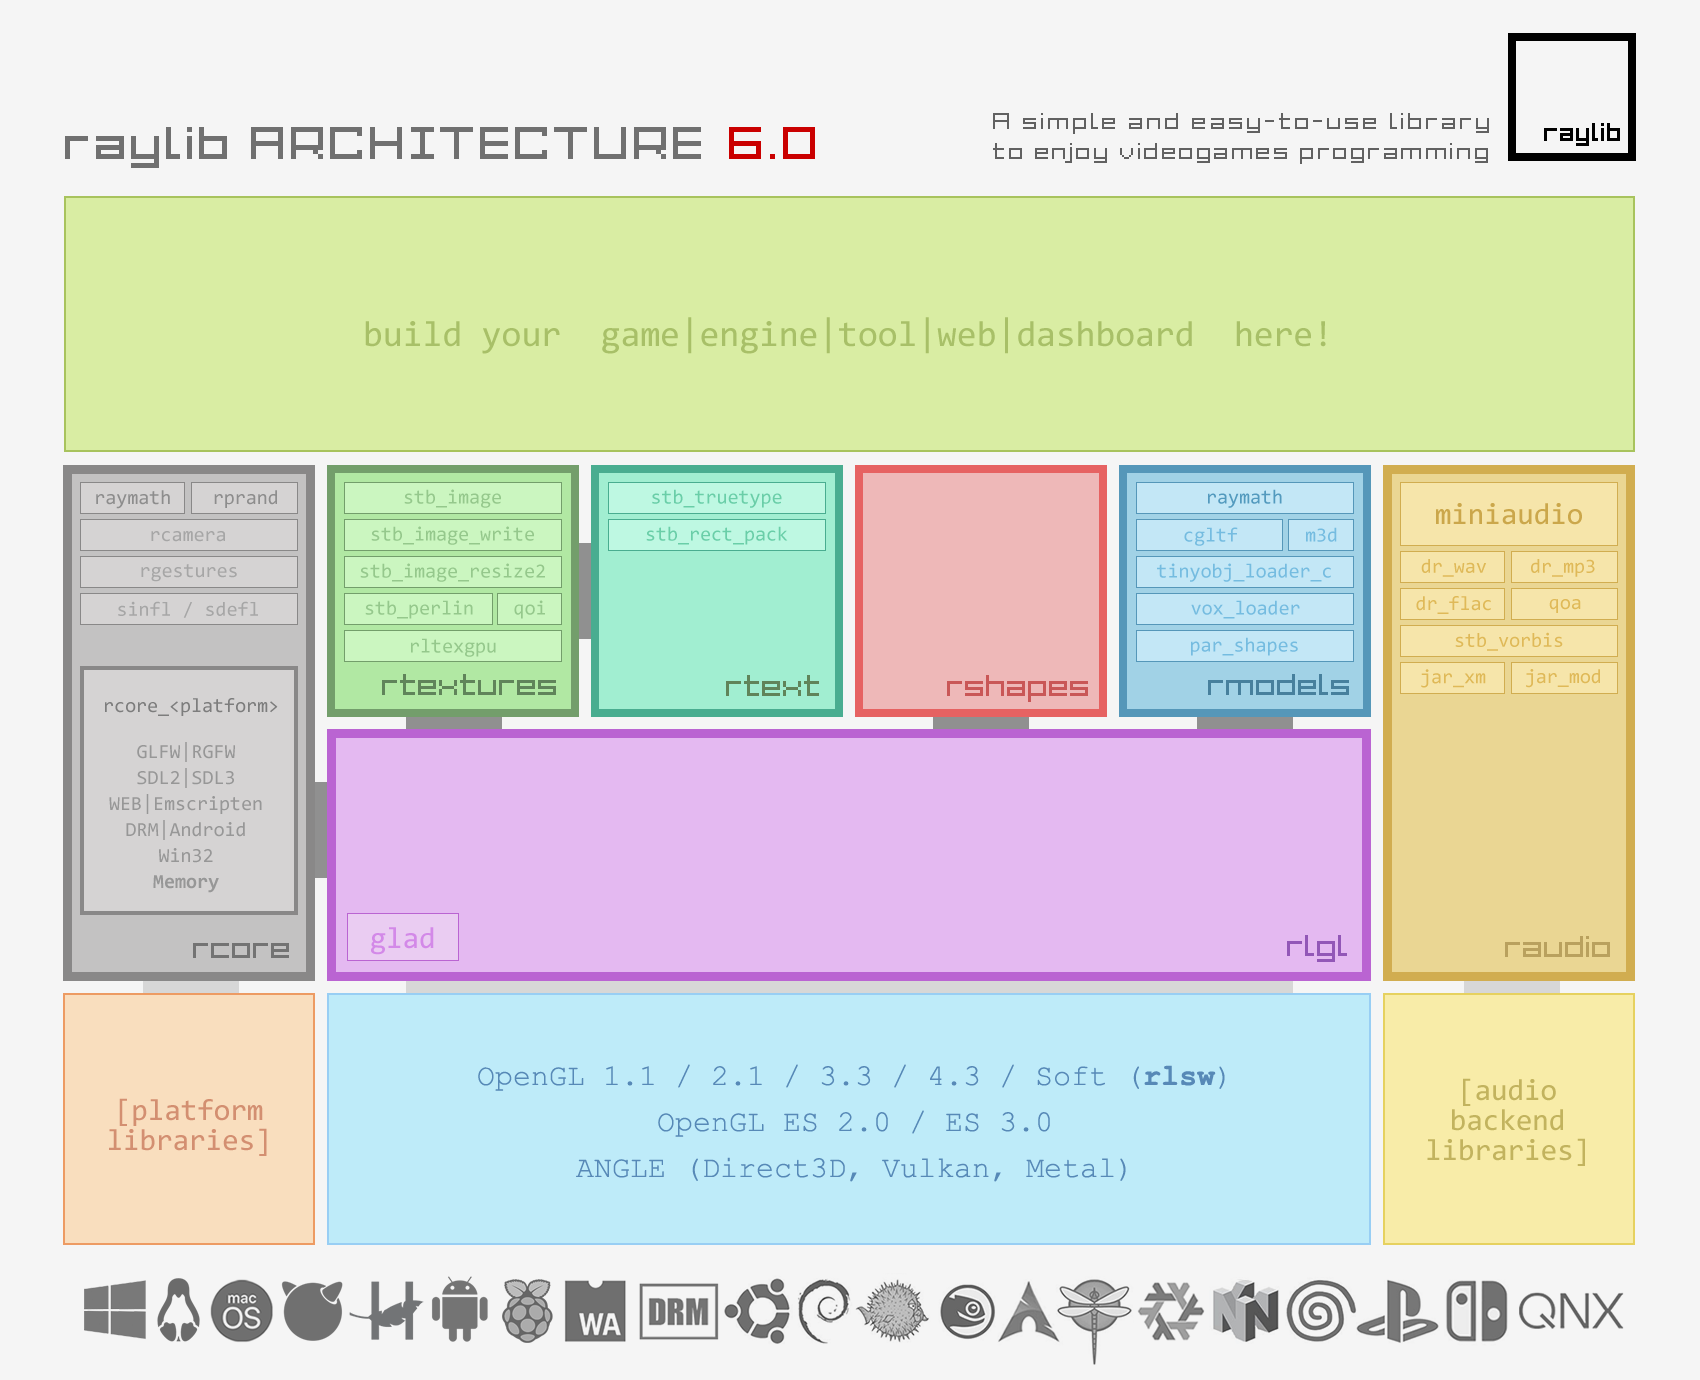
\includegraphics[width=0.85\textwidth]{imaxes/raylib_architecture_v6.0.png}
  \caption{Arquitectura de raylib}
  \label{fig:raylib-architecture}
\end{figure}

Esta organización por capas é a que lle permite ser fortemente multiplataforma.
Nos sistemas de escritorio, rcore delega a xestión da ventá, do contexto OpenGL e da entrada
en GLFW % \cite{glfw}
, unha librería multiplataforma que soporta Windows, macOS e Linux,
tanto baixo X11 como baixo Wayland.
Na web mantense a mesma interfaz:
o compilador Emscripten proporciona unha implementación da API de GLFW sobre o navegador,
na que a ventá pasa a ser un elemento canvas,
a entrada tradúcese a eventos do DOM
e as chamadas a OpenGL ES execútanse sobre WebGL,
todo iso co programa compilado a \acrfull{wasm}.
En sistemas embebidos GLFW substitúese por completo:
raylib pode renderizar mediante OpenGL ES sobre o subsistema \acrfull{drm} de Linux,
sen necesidade dun servidor gráfico,
e conta ademais cun renderizador por software para plataformas sen aceleración gráfica.
A comunidade mantén tamén adaptacións para consolas como a Nintendo 64.

A elección do backend realízase en tempo de compilación,
polo que o mesmo código fonte pode dirixirse a calquera destas plataformas sen modificacións.
Neste traballo a librería emprégase a través de raylib-rs % \cite{raylibrs}
, o seu binding para Rust, que expón estes backends como features de cargo
(por exemplo \texttt{raylib/wayland} ou \texttt{raylib/drm}),
o que permite que os frontends do emulador compilen para escritorio, web e embebidos
a partir do mesmo código.

\section{Outras ferramentas}

\subsection{Just como executor de tarefas}
Just % \cite{just}
é un executor de comandos semellante a make,
pero orientado a definir receitas de proxecto en lugar de xestionar dependencias entre ficheiros.
Nel centralízanse as tarefas habituais do proxecto:
a compilación, execución e comprobación do código, envolvendo a cargo;
o perfilado, a xeración da versión web, compilación cruzada...
As receitas len a variable \texttt{DISPLAY\_FEATURES} definida pola shell de Nix activa,
de forma que o mesmo comando compila para o backend gráfico correspondente a cada contorna.
Deste xeito os fluxos de traballo do proxecto quedan documentados no propio repositorio
e son compartidos entre diferentes desenvolvedores con contornas diferentes.


\subsection{Nix e as shells de desenvolvemento}
Nix % \cite{nix}
é un xestor de paquetes declarativo centrado na reproducibilidade.
Cada paquete descríbese como unha función pura das súas dependencias
e instálase nunha ruta illada e inmutable,
o que permite ter varias versións dunha mesma librería conviviendo sen conflitos.
Coas \textit{flakes}, as dependencias do propio proxecto decláranse nun ficheiro
e fíxanse a versións exactas nun \textit{lockfile},
de xeito que calquera máquina reproduce a mesma contorna co mesmo compilador e as mesmas librerías.

\subsubsection{Contornas de desenvolvemento}

Nix permítenos declarar como código as dependencias do proxecto
e xestionar o seu uso en diferentes contornas de desenvolvemento
, para evitar conflitos entre librerías incompatibles e mellorar a experiencia de desenvolvemento.
Este proxecto dispón de varias shells de desenvolvemento independentes para X11, Wayland, \acrshort{drm} e \acrshort{wasm},
que empregan as súas dependencias necesarias e exporta a variable de contorna \texttt{DISPLAY\_FEATURES} coas features de raylib correspondentes ao seu backend.
Ademais, tamén conta cunha shell para o desenvolvemento da memoria con \LaTeX{} en local.

% Por último, Nix emprégase tamén para xerar a imaxe completa do sistema operativo do dispositivo embebido:
% unha configuración mínima de NixOS a partir da que se constrúe unha imaxe de arranque
% para a Raspberry Pi empregada como plataforma de referencia, co emulador xa integrado.
% Deste xeito, non só a compilación senón tamén o despregue no hardware final é reproducible.

\subsection{Compilación cruzada}

\subsubsection{Contedores para as arquitecturas ARM}


\subsubsection{Compilación para a web con Emscripten}
A versión web constrúese co obxectivo \texttt{wasm32-unknown-emscripten}.
Emscripten % \cite{emscripten}
é unha cadea de ferramentas que compila código nativo a \acrshort{wasm}
e xera dous artefactos: o módulo WASM co código do programa
e un ficheiro JavaScript de "pegamento" 
que o carga no navegador e expón as funcións exportadas.

O proceso automatízase cunha receita de just
, compilando o frontend e copiando os artefactos cópianse a un directorio de distribución
xunto cos ficheiros estáticos da páxina.
que se pasa ao emulador a través do sistema de ficheiros virtual.
Para probar en local sérvese a páxina co módulo \texttt{http.server} de Python.

\section{Xustificación tecnolóxica}
Os obxectivos expostos na sección~\ref{sec:obxectivos} impoñen os requisitos 
sobre as tecnoloxías do proxecto:
o rendemento e a predicibilidade necesarios para emular a consola sobre hardware limitado,
a portabilidade dun núcleo en forma de librería integrable en contextos moi diferentes,
e un proceso de desenvolvemento e despregue reproducible en todas esas plataformas.

\subsection{Linguaxe de programación}
Rust é a linguaxe que mellor cobre os dous primeiros requisitos á vez.
As linguaxes tradicionais do ámbito, C e C++, ofrecen o mesmo rendemento.
A pesar de neste traballo no se aproveitar a súa capacidade para programación concurrente,
as garantías de seguridade de memoria de Rust permiten un desenvolvemento despreocupado
dos erros típicos de C e C++ que poden ser difíciles de detectar e depurar.
O sistema de tipos e \textit{pattern matching} permite modelar con claridade e de forma
óptima o hardware, o conxunto de instrucións e as máquinas de estado do emulador,
librando ao programador de posibles erros de implementación grazas á comprobación exhaustiva en compilación. 

\subsection{Librería gŕafica}
Na parte gráfica, a alternativa natural sería SDL, madura e igualmente multiplataforma.
Escolleuse raylib porque cobre vídeo, audio e entrada nunha única librería autocontida,
cunha API máis sinxela, soportando unha grande cantidade de plataformas.

En calquera caso, esta dependencia queda confinada nos frontends:
o núcleo do emulador non depende de raylib nin de ningunha outra librería.
Deste xeito, crear outro frontend empregando outra librería para outro contexto diferente
é trivial. O desenvolvedor só tería que implementar ás interfaces q demanda o emulador
e xa podería adecuar o resto do frontend ás súas necesidades.

As ferramentas restantes responden ao terceiro requisito.
Nix garante que todas as contornas de desenvolvemento son idénticas e reproducibles,
e fai viable traballar para catro backends gráficos incompatibles dende unha mesma máquina;
% os contedores con QEMU evitan manter cadeas de compilación cruzada fráxiles
% para producir binarios nativos do dispositivo embebido;
e just documenta e automatiza todos estes fluxos no propio repositorio.
Este apoio á reproducibilidade non é accesorio nun traballo coma este:
permite validar o emulador da mesma forma en todas as plataformas
e reforza a súa finalidade didáctica e documental,
xa que calquera persoa pode reproducir a contorna completa do proxecto e os seus resultados.
